%%%%%%%%%%%%%%%%%%%%%%%%%%%%%%%%%%%%%%%%%
% Stylish Article
% LaTeX Template
% Version 2.2 (2020-10-22)
%
% This template has been downloaded from:
% http://www.LaTeXTemplates.com
%
% Original author:
% Mathias Legrand (legrand.mathias@gmail.com) 
% With extensive modifications by:
% Vel (vel@latextemplates.com)
%
% License:
% CC BY-NC-SA 3.0 (http://creativecommons.org/licenses/by-nc-sa/3.0/)
%
%%%%%%%%%%%%%%%%%%%%%%%%%%%%%%%%%%%%%%%%%

%----------------------------------------------------------------------------------------
%	PACKAGES AND OTHER DOCUMENT CONFIGURATIONS
%----------------------------------------------------------------------------------------

\documentclass[fleqn,10pt]{SelfArx} % Document font size and equations flushed left

\usepackage[polish]{babel} % Specify a different language here - english by default
\usepackage[utf8]{inputenc} 	% W celu dekodowania polskich znaków
\usepackage[T1]{fontenc}
%\usepackage{polski}

\usepackage[bottom]{footmisc}	% Używamy, by stopka zawsze była na samym dole strony

\usepackage{lipsum} % Required to insert dummy text. To be removed otherwise

%----------------------------------------------------------------------------------------
%	COLUMNS
%----------------------------------------------------------------------------------------

\setlength{\columnsep}{0.55cm} % Distance between the two columns of text
\setlength{\fboxrule}{0.75pt} % Width of the border around the abstract

%----------------------------------------------------------------------------------------
%	COLORS
%----------------------------------------------------------------------------------------

\definecolor{color1}{RGB}{0,0,90} % Color of the article title and sections
\definecolor{color2}{RGB}{0,20,20} % Color of the boxes behind the abstract and headings

%----------------------------------------------------------------------------------------
%	HYPERLINKS
%----------------------------------------------------------------------------------------

\usepackage{hyperref} % Required for hyperlinks

\hypersetup{
	hidelinks,
	colorlinks,
	breaklinks=true,
	urlcolor=color2,
	citecolor=color1,
	linkcolor=color1,
	bookmarksopen=false,
	pdftitle={Title},
	pdfauthor={Author},
}

%----------------------------------------------------------------------------------------
%	ARTICLE INFORMATION
%----------------------------------------------------------------------------------------

\JournalInfo{Politechnika Poznańska, Poznań, \today} % Journal information
\Archive{Artykuł przeglądowy} % Additional notes (e.g. copyright, DOI, review/research article)

\PaperTitle{Przegląd ezoterycznych języków programowania} % Article title

\Authors{Mateusz Szuda\textsuperscript{1}} % Authors
\affiliation{\textsuperscript{1}\textit{student 3 roku Teleinformatyki, nr indeksu 144379, Politechnika Poznańska}} % Author affiliation

\Keywords{ezoteryczne --- języki --- programowania} % Keywords - if you don't want any simply remove all the text between the curly brackets
\newcommand{\keywordname}{Słowa kluczowe} % Defines the keywords heading name

%----------------------------------------------------------------------------------------
%	ABSTRACT - streszczenie
%----------------------------------------------------------------------------------------

\Abstract{
	Istnieje pewna grupa języków programowania zwana językami ezoterycznymi (ang. \textbf{\textit{esolang}}). \textit{Są one tworzone w celu badania i demonstracji niekonwencjonalnych technik programistycznych oraz metod programowania.
	Nie są one natomiast przeznaczone do pisania rzeczywistych aplikacji.}\cite{Wiki:EsotericPL}
	Ich twórcy skupiają się na dążeniu do stworzenia języka \textit{dziwnego} - \textbf{Malbolge}, \textit{minimalistycznego} - \textbf{Brainfuck}, \textit{o danym motywie} - \textbf{Shakespeare}, czy stworzonego dla \textit{zwykłego żartu} - \textbf{Ook!}.
	Zostało przedstawione tylko kilka przykładów języków oraz ich zastosowania, a w dalszej części artykułu poruszę kwestie związane z ich genezą,
	opiszę wymienione języki oraz zagłębię się w temat celów, jakimi kierowali się programiści podczas ich tworzenia. 
	Dodatkowo przedstawię semantykę tych języków okraszoną przykładowymi programami napisanymi za ich pomocą.
}

%----------------------------------------------------------------------------------------

\begin{document}

\maketitle % Output the title and abstract box

\tableofcontents % Output the contents section

\thispagestyle{empty} % Removes page numbering from the first page

%----------------------------------------------------------------------------------------
%	ARTICLE CONTENTS
%----------------------------------------------------------------------------------------

\section*{Wstęp} % The \section*{} command stops section numbering

\addcontentsline{toc}{section}{Wstęp} % Adds this section to the table of contents
	Opisując pojęcie \textit{języka programowania}, większość osób wyobraża sobie je jako narzędzie,
	zbiór zasad określających dane działania. Kod taki jest następnie kompilowany \textit{(np. C, C++)}, 
	bądź interpretowany \textit{(np. Python)} przez komputer, który wykonuje określone instrukcje zawarte w kodzie.
	Jednymi z najbardziej popularnych języków pozwalających nam na takie działania są: \underline{Python, Java, C, C++, JavaScript, C\#, R, Go}
	\cite{IEEESpectrum:popularLang2021}\footnote{wybór 8 najbardziej popularnych języków programowania w 2021 roku według serwisu IEEE spectrum:
	\url{https://spectrum.ieee.org/top-programming-languages-2021}}.
	Są to języki proste w swoim użyciu, zawierające bogatą i szeroko opisaną składnię językową. 
	Nie każdy język natomiast nadaje się do przetwarzania pewnych problemów, z którymi mierzą się programiści. 
	Program napisany w jednym języku może się wykonywać szybciej niż w drugim. To samo tyczy się objętości samych programów, 
	ich kompilatorów, czy samego kodu źródłowego. Dodatkowo należy mieć też na uwadze fakt, 
	iż jedne języki programowania są bardziej odpowiednie do rozwiązywania określonych zadań, konkretnych problemów, 
	w porównaniu do innych tworów.
	\indent Dobrym przykładem byłoby tutaj przywołanie grupy języków R, SQL i Matlab w opozycji do C, C++ i Javy. 
	Pierwsza grupa to języki przeznaczenia specjalistycznego, wykorzystywane do wszelakich obliczeń statystycznych, 
	czy algorytmicznych, reprezentacji graficznej wyników, czy wykonywania operacji bazodanowych. 
	Druga grupa są to języki ogólnego przeznaczenia, które pozwalają na stworzenie wysokowydajnych aplikacji, istniejące od wielu lat. 
	Ich niewątpliwą zaletą jest również fakt istnienia ogromnej bazy dokumentacji oraz aplikacji napisanych za pomocą tych języków. 
	\textit{W rzeczy samej, nawet znacząca część języka Python, jak i jego dokumentacji jest napisana w języku C z powodów wydajnościowych}
	\cite{IEEESpectrum:popularLang2021}\footnote{„Indeed, significant parts of Python itself and its libraries are written in C for performance reasons.” ~ \url{https://spectrum.ieee.org/top-programming-languages-2021}}.

%------------------------------------------------

\section{Czas na języki ezoteryczne}
	W momencie, gdy języki programowania są projektowane w celu produktywnego i efektywnego
	projektowania i budowania aplikacji, \textbf{języki ezoteryczne} tworzone są w innych celach: Mogą one reprezentować pewne idee \textbf{proof-of-concept},
	demonstrować \textbf{minimalizację} składni języka, który będzie nadal używalny, zachowując jednocześnie \textbf{uniwersalność}.
	Mogą one pomóc w udowodnieniu pewnych konceptów matematycznych, czy ustaleniu granic analiz złożoności.
	Proces projektowania języków ezoterycznych można zdefiniować jako operacja artystyczna,
	będąca wynikiem, a wręcz ekspresją ludzkiego intelektu, dowcipu, czy zmysłu \textcolor{red}{estetyki}.
	Mogą być również stworzone w celu podjęcia się swego rodzaju rywalizacji między programistami, bądź wyzwania, czy to dla siebie, czy dla hipotetycznego użytkownika.
	Istnieje jeszcze kolejna grupa języków ezoterycznych - języki prześmiewcze, napisanych ku uciesze autorów, użytkowników, czy choćby czytelników ich specyfikacji.\cite{morr2015esoteric}
	Wszystkie wymienione właściwości, jak i charakterystyki języków ezoterycznych wywołują chęć przyjrzenia się im dokładniej oraz poznania zamiarów ekscentrycznych programistów stojących za ich powstaniem.

%------------------------------------------------
% TODO: rodzaje języków? (na WIKI jest rozpiska)


\section{Methods}

\begin{figure*}[ht]\centering % Using \begin{figure*} makes the figure take up the entire width of the page
	
\includegraphics[width=\linewidth]{view}
	\caption{Wide Picture}
	\label{fig:view}
\end{figure*}

\lipsum[4] % Dummy text

\begin{equation}
	\cos^3 \theta =\frac{1}{4}\cos\theta+\frac{3}{4}\cos 3\theta
	\label{eq:refname2}
\end{equation}

\lipsum[5] % Dummy text

\begin{enumerate}[noitemsep] % [noitemsep] removes whitespace between the items for a compact look
	\item First item in a list
	\item Second item in a list
	\item Third item in a list
\end{enumerate}

\subsection{Subsection}

\lipsum[6] % Dummy text

\paragraph{Paragraph} \lipsum[7] % Dummy text
\paragraph{Paragraph} \lipsum[8] % Dummy text

\subsection{Subsection}

\lipsum[9] % Dummy text

\begin{figure}[ht]\centering
	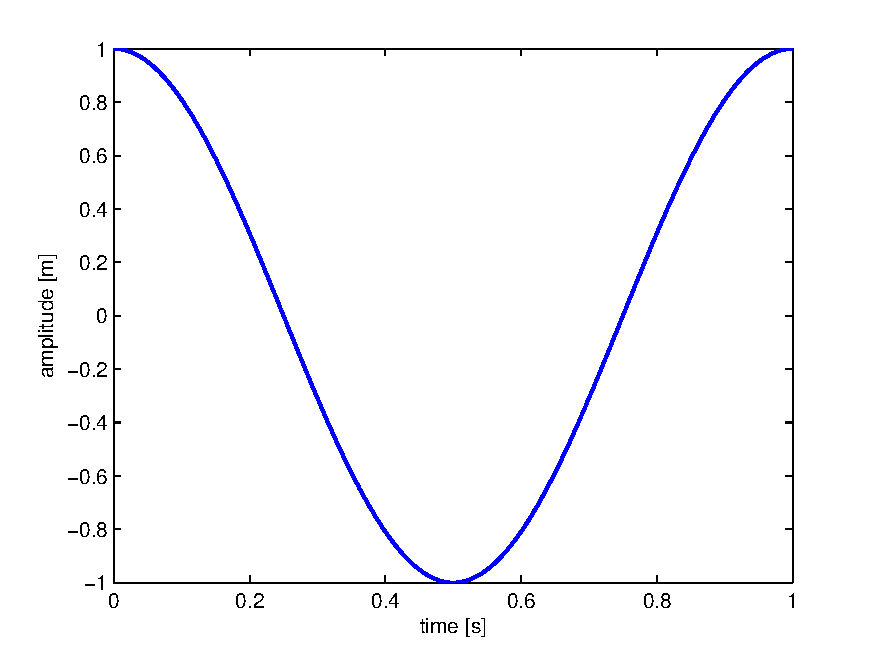
\includegraphics[width=\linewidth]{results}
	\caption{In-text Picture}
	\label{fig:results}
\end{figure}

Reference to Figure \ref{fig:results}.

%------------------------------------------------

\section{Results and Discussion}

\lipsum[10] % Dummy text

\subsection{Subsection}

\lipsum[11] % Dummy text

\begin{table}[hbt]
	\caption{Table of Grades}
	\centering
	\begin{tabular}{llr}
		\toprule
		\multicolumn{2}{c}{Name} \\
		\cmidrule(r){1-2}
		First name & Last Name & Grade \\
		\midrule
		John & Doe & $7.5$ \\
		Richard & Miles & $2$ \\
		\bottomrule
	\end{tabular}
	\label{tab:label}
\end{table}

\subsubsection{Subsubsection}

\lipsum[12] % Dummy text

\begin{description}
	\item[Word] Definition
	\item[Concept] Explanation
	\item[Idea] Text
\end{description}

\subsubsection{Subsubsection}

\lipsum[13] % Dummy text

\begin{itemize}[noitemsep] % [noitemsep] removes whitespace between the items for a compact look
	\item First item in a list
	\item Second item in a list
	\item Third item in a list
\end{itemize}

\subsubsection{Subsubsection}

\lipsum[14] % Dummy text

\subsection{Subsection}

\lipsum[15-23] % Dummy text

%------------------------------------------------

\phantomsection
\section*{Acknowledgments} % The \section*{} command stops section numbering

\addcontentsline{toc}{section}{Acknowledgments} % Adds this section to the table of contents

So long and thanks for all the fish \cite{Figueredo:2009dg, Smith:2012qr}.

%----------------------------------------------------------------------------------------
%	REFERENCE LIST
%----------------------------------------------------------------------------------------

\phantomsection
\bibliographystyle{unsrt}
\bibliography{bibliography.bib}

%----------------------------------------------------------------------------------------

\end{document}